% Vietnamese translation for OI Public Library
% Source-PDF: IOI中国国家候选队论文/2007/day1/10.陈启峰《Size Balanced Tree》.pdf
\documentclass[11pt]{article}
\usepackage{oipl-vn}
\usepackage{tikz}
\usetikzlibrary{arrows.meta}

\newcommand{\Oh}{\mathcal{O}}
\tikzset{
  sbt node/.style={
    circle,draw=green!45!black,fill=black!18,minimum size=0.62cm,
    inner sep=0pt,font=\small
  },
  sbt edge/.style={black!75,line width=0.45pt},
  sbt leaf/.style={draw=violet!70!black,fill=black!12,line width=0.45pt}
}
\newcommand{\sbtleafat}[2]{%
  \begin{scope}[shift={(#1)}]
    \draw[sbt leaf] (0,0.42)--(-0.45,-0.32)--(0.45,-0.32)--cycle;
    \node[font=\small] at (0,-0.02) {$#2$};
  \end{scope}%
}

\title{Size Balanced Tree}
\author{Chen Qifeng (Farmer John)}
\date{29 tháng 12 năm 2006}

\begin{document}
\maketitle

\origtitle{Size Balanced Tree}
\sourcepath{IOI China candidate team papers / 2007 / day 1 / Chen Qifeng}

\begin{center}
Zhongshan Memorial Middle School, Guangdong, China

Email: \texttt{344368722@QQ.com}
\end{center}

\section*{Tóm tắt}

Bài viết trình bày một chiến lược độc đáo để duy trì cân bằng trong cây tìm
kiếm nhị phân thay đổi động, với hành vi kỳ vọng tối ưu ngay cả trong trường
hợp xấu nhất. Đúng như tên gọi, \term{Size Balanced Tree} là cây tìm kiếm nhị
phân được giữ cân bằng bằng kích thước. Nó đơn giản, hiệu quả và linh hoạt về
mọi mặt. Cài đặt rất dễ, mô tả trực tiếp, đồng thời chứng minh tính đúng đắn
và thời gian chạy cũng đơn giản một cách đáng ngạc nhiên. Thời gian chạy của
nó ngang với những cây tìm kiếm nhị phân nhanh nhất đã biết. Hơn nữa, trong
thực tế nó thường nhanh hơn nhiều cây tìm kiếm nhị phân cân bằng nổi tiếng
khác vì có xu hướng tiến gần đến cây cân bằng hoàn hảo. Nó không chỉ hỗ trợ
các thao tác cơ bản điển hình mà còn hỗ trợ \textsc{Select} và \textsc{Rank}.

\paragraph{Từ khóa.}
Size Balanced Tree; SBT; duy trì cân bằng.

\begin{center}
\textit{Bài viết này được dành để tưởng nhớ Heavens.}
\end{center}

\section{Dẫn nhập}

Trước khi trình bày Size Balanced Tree, cần nhắc lại cây tìm kiếm nhị phân và
hai phép quay trên cây tìm kiếm nhị phân: quay trái và quay phải.

\subsection{Cây tìm kiếm nhị phân}

Cây tìm kiếm nhị phân là một loại cấu trúc dữ liệu nâng cao quan trọng. Nó hỗ
trợ nhiều thao tác trên tập động, gồm \textsc{Search}, \textsc{Minimum},
\textsc{Maximum}, \textsc{Predecessor}, \textsc{Successor}, \textsc{Insert}
và \textsc{Delete}. Nó có thể được dùng như một từ điển hoặc một hàng đợi ưu
tiên.

Một cây tìm kiếm nhị phân (viết tắt là BST) là một cây nhị phân có tổ chức.
Mỗi nút trong BST có nhiều nhất hai con. Các khóa dùng để so sánh trong BST
luôn được lưu sao cho thỏa tính chất cây tìm kiếm nhị phân:

\begin{quote}
Với một nút $x$ trong cây tìm kiếm nhị phân, khóa của $x$ không nhỏ hơn các
khóa trong cây con trái và không lớn hơn các khóa trong cây con phải.
\end{quote}

Với mỗi nút $t$, ta dùng các trường $\mathit{left}[t]$ và $\mathit{right}[t]$
để lưu hai con trỏ đến con của nó. Ta định nghĩa $\mathit{key}[t]$ là giá trị
của nút $t$ dùng cho so sánh. Ngoài ra, ta thêm $s[t]$, kích thước của cây con
gốc $t$, để lưu số nút trong cây ấy. Đặc biệt, ta gọi $0$ là con trỏ đến cây
rỗng và đặt $s[0]=0$.

\subsection{Phép quay}

Để giữ BST cân bằng, tức không suy biến thành một dây xích, ta thường thay
đổi cấu trúc con trỏ bằng các phép quay. Phép quay là thao tác cục bộ trong
cây tìm kiếm, giữ nguyên tính chất cây tìm kiếm nhị phân nhưng thay đổi hình
dạng cây.

\begin{center}
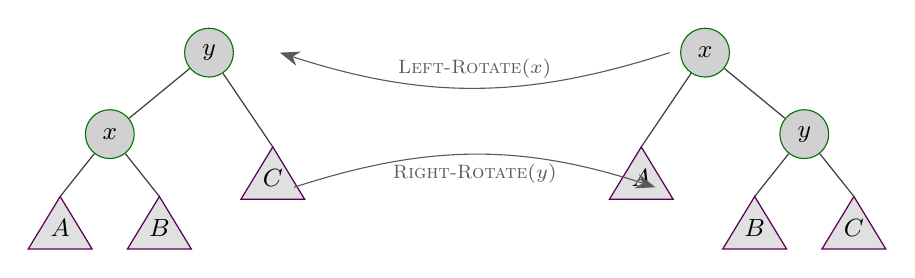
\begin{tikzpicture}[x=0.9cm,y=0.9cm]
  \node[sbt node] (ly) at (0,1.8) {$y$};
  \node[sbt node] (lx) at (-1.4,0.65) {$x$};
  \sbtleafat{-2.1,-0.65}{A}
  \sbtleafat{-0.7,-0.65}{B}
  \sbtleafat{0.9,0.05}{C}
  \draw[sbt edge] (ly)--(lx) (ly)--(0.9,0.47)
    (lx)--(-2.1,-0.23) (lx)--(-0.7,-0.23);

  \node[sbt node] (rx) at (7,1.8) {$x$};
  \node[sbt node] (ry) at (8.4,0.65) {$y$};
  \sbtleafat{6.1,0.05}{A}
  \sbtleafat{7.7,-0.65}{B}
  \sbtleafat{9.1,-0.65}{C}
  \draw[sbt edge] (rx)--(6.1,0.47) (rx)--(ry)
    (ry)--(7.7,-0.23) (ry)--(9.1,-0.23);

  \draw[-{Stealth[length=2.5mm]},black!65] (6.5,1.8) to[bend left=18]
    node[above,font=\scriptsize]{\textsc{Left-Rotate}$(x)$} (1.0,1.8);
  \draw[-{Stealth[length=2.5mm]},black!65] (1.2,-0.1) to[bend left=18]
    node[below,font=\scriptsize]{\textsc{Right-Rotate}$(y)$} (6.3,-0.1);
\end{tikzpicture}\\[-0.2em]
{\small Hình 1.1. Hai phép quay trái và quay phải là nghịch đảo của nhau.}
\end{center}

\subsubsection{Mã giả của quay phải}

Phép quay phải giả thiết rằng con trái tồn tại.

\begin{verbatim}
Right-Rotate(t)
1  k <- left[t]
2  left[t] <- right[k]
3  right[k] <- t
4  s[k] <- s[t]
5  s[t] <- s[left[t]] + s[right[t]] + 1
6  t <- k
\end{verbatim}

\subsubsection{Mã giả của quay trái}

Phép quay trái giả thiết rằng con phải tồn tại.

\begin{verbatim}
Left-Rotate(t)
1  k <- right[t]
2  right[t] <- left[k]
3  left[k] <- t
4  s[k] <- s[t]
5  s[t] <- s[left[t]] + s[right[t]] + 1
6  t <- k
\end{verbatim}

\section{Size Balanced Tree}

Size Balanced Tree (viết tắt là SBT) là một loại cây tìm kiếm nhị phân được
giữ cân bằng bằng kích thước. Nó hỗ trợ nhiều thao tác động cơ bản trong thời
gian $\Oh(\log n)$:

\begin{description}
  \item[\textsc{Insert}$(t,v)$] Chèn một nút có khóa $v$ vào SBT gốc $t$.
  \item[\textsc{Delete}$(t,v)$] Xóa một nút có khóa $v$ khỏi SBT gốc $t$.
  Nếu trong cây không có nút như vậy, xóa nút được tìm thấy cuối cùng.
  \item[\textsc{Find}$(t,v)$] Tìm nút có khóa $v$ và trả về nút đó.
  \item[\textsc{Rank}$(t,v)$] Trả về hạng của $v$ trong cây gốc $t$. Nói cách
  khác, đây là một cộng với số khóa nhỏ hơn $v$ trong cây ấy.
  \item[\textsc{Select}$(t,k)$] Trả về nút đứng ở vị trí thứ $k$. Rõ ràng thao
  tác này bao gồm cả lấy phần tử nhỏ nhất và lớn nhất, vì
  \textsc{Get-Min} tương đương \textsc{Select}$(t,1)$, còn \textsc{Get-Max}
  tương đương \textsc{Select}$(t,s[t])$.
  \item[\textsc{Pred}$(t,v)$] Trả về nút có khóa lớn nhất nhưng nhỏ hơn $v$.
  \item[\textsc{Succ}$(t,v)$] Trả về nút có khóa nhỏ nhất nhưng lớn hơn $v$.
\end{description}

Thông thường mỗi nút của SBT chứa khóa, con trái, con phải và một trường phụ
nhưng hữu ích luôn được cập nhật: kích thước của nó, như đã định nghĩa ở
phần trên. Cốt lõi của SBT gồm hai ràng buộc theo kích thước:

\begin{quote}
Với mọi nút được trỏ bởi $t$ trong SBT, ta bảo đảm:
\[
\tag{a}
s[\mathit{right}[t]] \ge
s[\mathit{left}[\mathit{left}[t]]],\quad
s[\mathit{right}[t]] \ge
s[\mathit{right}[\mathit{left}[t]]],
\]
\[
\tag{b}
s[\mathit{left}[t]] \ge
s[\mathit{right}[\mathit{right}[t]]],\quad
s[\mathit{left}[t]] \ge
s[\mathit{left}[\mathit{right}[t]]].
\]
\end{quote}

Trong Hình 2.1, các nút $L$ và $R$ lần lượt là con trái và con phải của nút
$T$. Các cây con $A,B$ lần lượt là cây con trái và phải của $L$; các cây con
$C,D$ lần lượt là cây con trái và phải của $R$. Tương ứng với hai tính chất
(a) và (b), ta có
\[
  s[A],s[B]\le s[R],
  \qquad
  s[C],s[D]\le s[L].
\]

\begin{center}
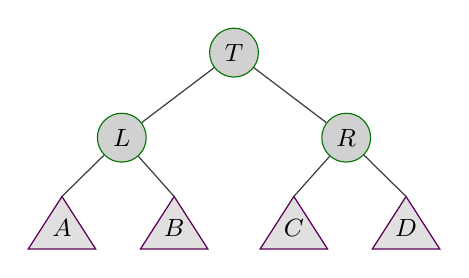
\begin{tikzpicture}[x=0.95cm,y=0.9cm]
  \node[sbt node] (t) at (0,2.2) {$T$};
  \node[sbt node] (l) at (-1.5,1.0) {$L$};
  \node[sbt node] (r) at (1.5,1.0) {$R$};
  \sbtleafat{-2.3,-0.25}{A}
  \sbtleafat{-0.8,-0.25}{B}
  \sbtleafat{0.8,-0.25}{C}
  \sbtleafat{2.3,-0.25}{D}
  \draw[sbt edge] (t)--(l) (t)--(r)
    (l)--(-2.3,0.17) (l)--(-0.8,0.17)
    (r)--(0.8,0.17) (r)--(2.3,0.17);
\end{tikzpicture}\\[-0.2em]
{\small Hình 2.1. Ký hiệu các cây con quanh nút $T$.}
\end{center}

\section{Duy trì cân bằng}

Giả sử ta cần chèn một nút có khóa $v$ vào một BST. Thông thường ta dùng thủ
tục sau:

\begin{verbatim}
Simple-Insert(t, v)
1  If t = 0 then
2      t <- NEW-NODE(v)
3  Else
4      s[t] <- s[t] + 1
5      If v < key[t] then
6          Simple-Insert(left[t], v)
7      Else
8          Simple-Insert(right[t], v)
\end{verbatim}

Sau khi thực hiện \textsc{Simple-Insert}, các tính chất (a) và (b) có thể
không còn thỏa. Khi đó ta cần duy trì lại SBT.

Thao tác then chốt trên SBT là một thủ tục duy nhất: \textsc{Maintain}.
\textsc{Maintain}$(t)$ được dùng để duy trì SBT gốc $t$. Trước khi gọi thủ
tục này, giả thiết là các cây con của $t$ đã là SBT.

Vì hai tính chất (a) và (b) đối xứng nhau, ta chỉ thảo luận chi tiết trường
hợp ràng buộc (a) bị vi phạm.

\subsection*{Trường hợp 1: $s[\mathit{left}[\mathit{left}[t]]]>s[\mathit{right}[t]]$}

Trong trường hợp $s[A]>s[R]$ tương ứng với hình 2.1 sau khi chèn vào
$\mathit{left}[t]$, ta có thể sửa SBT bằng các bước sau:

\begin{enumerate}
  \item Trước hết thực hiện \textsc{Right-Rotate}$(T)$. Thao tác này biến cấu
  hình của hình 2.1 thành cấu hình của hình 3.1.
\begin{center}
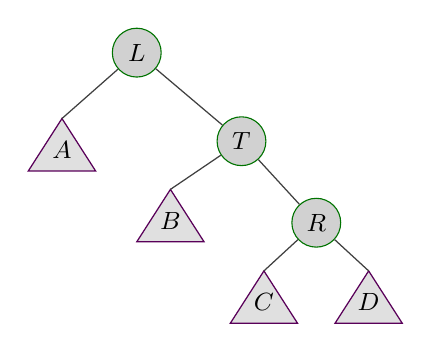
\begin{tikzpicture}[x=0.95cm,y=0.9cm]
  \node[sbt node] (l) at (0,2.5) {$L$};
  \node[sbt node] (t) at (1.4,1.25) {$T$};
  \node[sbt node] (r) at (2.4,0.1) {$R$};
  \sbtleafat{-1.0,1.15}{A}
  \sbtleafat{0.45,0.15}{B}
  \sbtleafat{1.7,-1.0}{C}
  \sbtleafat{3.1,-1.0}{D}
  \draw[sbt edge] (l)--(-1.0,1.57) (l)--(t)
    (t)--(0.45,0.57) (t)--(r)
    (r)--(1.7,-0.58) (r)--(3.1,-0.58);
\end{tikzpicture}\\[-0.2em]
{\small Hình 3.1. Kết quả sau \textsc{Right-Rotate}$(T)$.}
\end{center}
  \item Đôi khi cây vẫn chưa là SBT, vì có thể xảy ra $s[C]>s[B]$ hoặc
  $s[D]>s[B]$. Do đó cần thực hiện \textsc{Maintain}$(T)$.
  \item Sau đó, cấu hình cây con phải của nút $L$ có thể đã thay đổi. Vì vẫn
  có khả năng vi phạm tính chất cân bằng, cần chạy lại \textsc{Maintain}$(L)$.
\end{enumerate}

\subsection*{Trường hợp 2: $s[\mathit{right}[\mathit{left}[t]]]>s[\mathit{right}[t]]$}

Trong trường hợp $s[B]>s[R]$ tương ứng với hình 3.2 sau khi chèn vào
$\mathit{left}[t]$, việc duy trì phức tạp hơn trường hợp 1 một chút. Ta có
thể sửa bằng các thao tác sau.

\begin{center}
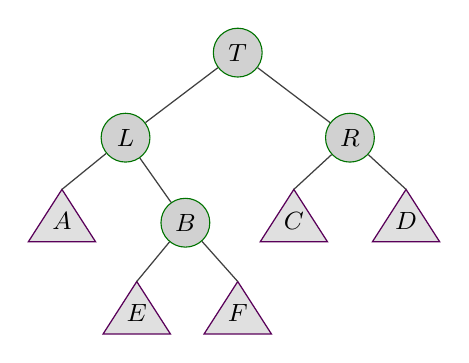
\begin{tikzpicture}[x=0.95cm,y=0.9cm]
  \node[sbt node] (t) at (0,3.2) {$T$};
  \node[sbt node] (l) at (-1.5,2.0) {$L$};
  \node[sbt node] (r) at (1.5,2.0) {$R$};
  \node[sbt node] (b) at (-0.7,0.8) {$B$};
  \sbtleafat{-2.35,0.85}{A}
  \sbtleafat{-1.35,-0.45}{E}
  \sbtleafat{0.0,-0.45}{F}
  \sbtleafat{0.75,0.85}{C}
  \sbtleafat{2.25,0.85}{D}
  \draw[sbt edge] (t)--(l) (t)--(r)
    (l)--(-2.35,1.27) (l)--(b)
    (b)--(-1.35,-0.03) (b)--(0.0,-0.03)
    (r)--(0.75,1.27) (r)--(2.25,1.27);
\end{tikzpicture}\\[-0.2em]
{\small Hình 3.2. Trường hợp $B$ là cây con phải của $L$.}
\end{center}

\begin{enumerate}
  \item Trước hết thực hiện \textsc{Left-Rotate}$(L)$. Sau thao tác này, cấu
  hình hình 3.2 được biến thành cấu hình hình 3.3.
\begin{center}
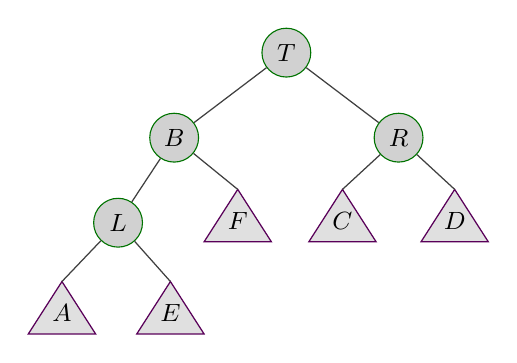
\begin{tikzpicture}[x=0.95cm,y=0.9cm]
  \node[sbt node] (t) at (0,3.2) {$T$};
  \node[sbt node] (b) at (-1.5,2.0) {$B$};
  \node[sbt node] (r) at (1.5,2.0) {$R$};
  \node[sbt node] (l) at (-2.25,0.8) {$L$};
  \sbtleafat{-3.0,-0.45}{A}
  \sbtleafat{-1.55,-0.45}{E}
  \sbtleafat{-0.65,0.85}{F}
  \sbtleafat{0.75,0.85}{C}
  \sbtleafat{2.25,0.85}{D}
  \draw[sbt edge] (t)--(b) (t)--(r)
    (b)--(l) (b)--(-0.65,1.27)
    (l)--(-3.0,-0.03) (l)--(-1.55,-0.03)
    (r)--(0.75,1.27) (r)--(2.25,1.27);
\end{tikzpicture}\\[-0.2em]
{\small Hình 3.3. Kết quả sau \textsc{Left-Rotate}$(L)$.}
\end{center}
  \item Tiếp theo thực hiện \textsc{Right-Rotate}$(T)$. Thao tác này biến hình
  3.3 thành hình 3.4.
\begin{center}
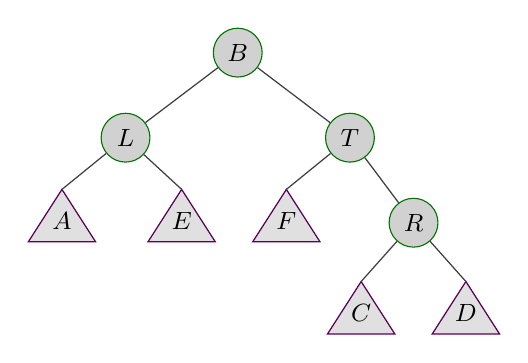
\begin{tikzpicture}[x=0.95cm,y=0.9cm]
  \node[sbt node] (b) at (0,3.2) {$B$};
  \node[sbt node] (l) at (-1.5,2.0) {$L$};
  \node[sbt node] (t) at (1.5,2.0) {$T$};
  \node[sbt node] (r) at (2.35,0.8) {$R$};
  \sbtleafat{-2.35,0.85}{A}
  \sbtleafat{-0.75,0.85}{E}
  \sbtleafat{0.65,0.85}{F}
  \sbtleafat{1.65,-0.45}{C}
  \sbtleafat{3.05,-0.45}{D}
  \draw[sbt edge] (b)--(l) (b)--(t)
    (l)--(-2.35,1.27) (l)--(-0.75,1.27)
    (t)--(0.65,1.27) (t)--(r)
    (r)--(1.65,-0.03) (r)--(3.05,-0.03);
\end{tikzpicture}\\[-0.2em]
{\small Hình 3.4. Kết quả sau \textsc{Right-Rotate}$(T)$.}
\end{center}
  \item Sau hai phép quay, cây trở nên khó đoán hơn. May mắn là trong hình
  3.4, các cây con $A,E,F,R$ vẫn là SBT. Vì vậy ta có thể thực hiện
  \textsc{Maintain}$(L)$ và \textsc{Maintain}$(T)$ để sửa hai cây con của nút
  $B$.
  \item Sau bước trên, các cây con ấy đã là SBT. Nhưng tại nút $B$, các tính
  chất (a) và (b) vẫn có thể bị vi phạm. Do đó cần thực hiện lại
  \textsc{Maintain}$(B)$.
\end{enumerate}

\subsection*{Trường hợp 3: $s[\mathit{right}[\mathit{right}[t]]]>s[\mathit{left}[t]]$}

Trường hợp này đối xứng với trường hợp 1.

\subsection*{Trường hợp 4: $s[\mathit{left}[\mathit{right}[t]]]>s[\mathit{left}[t]]$}

Trường hợp này đối xứng với trường hợp 2.

\subsection{Mã giả của \textsc{Maintain} chuẩn}

Theo phân tích trên, ta dễ dàng cài đặt một thủ tục \textsc{Maintain} thông
thường.

\begin{verbatim}
Maintain(t)
1   If s[left[left[t]]] > s[right[t]] then
2       Right-Rotate(t)
3       Maintain(right[t])
4       Maintain(t)
5       Exit
6   If s[right[left[t]]] > s[right[t]] then
7       Left-Rotate(left[t])
8       Right-Rotate(t)
9       Maintain(left[t])
10      Maintain(right[t])
11      Maintain(t)
12      Exit
13  If s[right[right[t]]] > s[left[t]] then
14      Left-Rotate(t)
15      Maintain(left[t])
16      Maintain(t)
17      Exit
18  If s[left[right[t]]] > s[left[t]] then
19      Right-Rotate(right[t])
20      Left-Rotate(t)
21      Maintain(left[t])
22      Maintain(right[t])
23      Maintain(t)
\end{verbatim}

\subsection{Mã giả của \textsc{Maintain} nhanh hơn và đơn giản hơn}

Mã giả chuẩn hơi phức tạp và chậm. Thông thường ta có thể biết trước rằng
tính chất (a) hoặc (b) đã thỏa. Vì vậy chỉ cần kiểm tra các trường hợp 1, 2
hoặc các trường hợp 3, 4 để tăng tốc. Khi đó ta thêm một biến Boolean
\textit{flag} để tránh các kiểm tra vô nghĩa. Nếu \textit{flag} là
\textit{false}, ta kiểm tra trường hợp 1 và 2; ngược lại ta kiểm tra trường
hợp 3 và 4.

\begin{verbatim}
Maintain(t, flag)
1   If flag = false then
2       If s[left[left[t]]] > s[right[t]] then
3           Right-Rotate(t)
4       Elseif s[right[left[t]]] > s[right[t]] then
5           Left-Rotate(left[t])
6           Right-Rotate(t)
7       Else exit
8   Elseif s[right[right[t]]] > s[left[t]] then
9       Left-Rotate(t)
10  Elseif s[left[right[t]]] > s[left[t]] then
11      Right-Rotate(right[t])
12      Left-Rotate(t)
13  Else exit
14  Maintain(left[t], false)
15  Maintain(right[t], true)
16  Maintain(t, false)
17  Maintain(t, true)
\end{verbatim}

Vì sao có thể bỏ \textsc{Maintain}$(\mathit{left}[t],\textit{true})$ và
\textsc{Maintain}$(\mathit{right}[t],\textit{false})$? Thời gian chạy của
\textsc{Maintain} là bao nhiêu? Câu trả lời nằm ở phần 6, phân tích.

\section{Chèn}

Thao tác chèn trên SBT rất đơn giản. Sau đây là mã giả của \textsc{Insert}
trên SBT.

\subsection{Mã giả của \textsc{Insert}}

\begin{verbatim}
Insert(t, v)
1  If t = 0 then
2      t <- NEW-NODE(v)
3  Else
4      s[t] <- s[t] + 1
5      If v < key[t] then
6          Simple-Insert(left[t], v)
7      Else
8          Simple-Insert(right[t], v)
9      Maintain(t, v >= key[t])
\end{verbatim}

\section{Xóa}

Tác giả mở rộng thao tác xóa cho tiện dùng. Nếu giá trị cần xóa không tồn tại
trong SBT, ta xóa nút được tìm thấy cuối cùng và ghi lại nó. Sau đây là mã
giả chuẩn của \textsc{Delete} trên SBT.

\subsection{Mã giả của \textsc{Delete} chuẩn}

\begin{verbatim}
Delete(t, v)
1  If s[t] <= 2 then
2      record <- key[t]
3      t <- left[t] + right[t]
4      Exit
5  s[t] <- s[t] - 1
6  If v = key[t] then
7      Delete(left[t], v[t] + 1)
8      key[t] <- record
9      Maintain(t, true)
10 Else
11     If v < key[t] then
12         Delete(left[t], v)
13     Else
14         Delete(right[t], v)
15     Maintain(t, v < key[t])
\end{verbatim}

\subsection{Mã giả của \textsc{Delete} nhanh hơn và đơn giản hơn}

Thực ra đây là thao tác xóa đơn giản nhất mà không cần hàm phụ khác. Ở đây
\textsc{Delete}$(t,v)$ là một hàm trả về giá trị bị xóa. Nó có thể làm hỏng
cấu trúc SBT. Nhưng khi dùng cùng thao tác chèn ở trên, BST vẫn được giữ ở độ
cao $\Oh(\log n^*)$, trong đó $n^*$ là tổng số lần chèn, chứ không phải kích
thước hiện tại.

\begin{verbatim}
Delete(t, v)
1  s[t] <- s[t] - 1
2  If (v = key[t]) or (v < key[t]) and (left[t] = 0) or
      (v > key[t]) and (right[t] = 0) then
3      Delete <- key[t]
4      If (left[t] = 0) or (right[t] = 0) then
5          t <- left[t] + right[t]
6      Else
7          key[t] <- Delete(left[t], v[t] + 1)
8  Else
9      If v < key[t] then
10         Delete(left[t], v)
11     Else
12         Delete(right[t], v)
\end{verbatim}

\section{Phân tích}

Rõ ràng \textsc{Maintain} là một thủ tục đệ quy. Có thể bạn sẽ tự hỏi liệu
nó có dừng hay không. Không cần lo: người ta đã chứng minh được rằng thời gian
khấu hao của \textsc{Maintain} chỉ là $\Oh(1)$.

\subsection{Phân tích độ cao}

Gọi $f[h]$ là số nút nhỏ nhất của một SBT có độ cao $h$. Ta có
\[
f[h]=
\begin{cases}
1, & h=0,\\
2, & h=1,\\
f[h-1]+f[h-2]+1, & h>1.
\end{cases}
\]

\subsubsection{Chứng minh}

\begin{enumerate}
  \item Dễ thấy $f[0]=1$ và $f[1]=2$.
  \item Trước hết,
  \[
    f[h]\ge f[h-1]+f[h-2]+1 \qquad (h>1).
  \]
  Với mỗi $h>1$, giả sử $t$ trỏ đến một SBT có độ cao $h$. Khi đó SBT này
  chứa một cây con có độ cao $h-1$. Không mất tính tổng quát, giả sử đó là
  cây con trái. Theo định nghĩa của $f[h]$, ta có
  $s[\mathit{left}[t]]\ge f[h-1]$. Trong cây con trái ấy có một cây con cao
  $h-2$, nói cách khác có một cây con kích thước ít nhất $f[h-2]$. Nhờ tính
  chất (b), ta có $s[\mathit{right}[t]]\ge f[h-2]$. Vì vậy
  \[
    s[t]\ge f[h-1]+f[h-2]+1.
  \]

  Mặt khác,
  \[
    f[h]\le f[h-1]+f[h-2]+1 \qquad (h>1).
  \]
  Ta có thể xây dựng một SBT đúng $f[h]$ nút và có độ cao $h$. Gọi loại SBT
  này là $\mathit{tree}[h]$:
  \[
  \mathit{tree}[h]=
  \begin{cases}
  \text{một BST có một nút}, & h=0,\\
  \text{một BST bất kỳ có hai nút}, & h=1,\\
  \text{một BST chứa }\mathit{tree}[h-1]\text{ và }\mathit{tree}[h-2]
  \text{ làm hai cây con}, & h>1.
  \end{cases}
  \]
  Tổng hợp hai phía trên, ta thu được
  $f[h]=f[h-1]+f[h-2]+1$ với $h>1$.
\end{enumerate}

\subsubsection{Độ cao xấu nhất}

Thực ra $f[h]$ là hàm mũ. Giá trị chính xác của nó có thể tính từ truy hồi:
\[
f[h]
=\frac{\alpha^{h+3}-\beta^{h+3}}{\sqrt{5}}-1
=\frac{\alpha^{h+3}}{\sqrt{5}}-1
=\operatorname{Fibonacci}[h+2]-1
=\sum_{i=0}^{h}\operatorname{Fibonacci}[i],
\]
trong đó
\[
  \alpha=\frac{1+\sqrt{5}}{2},
  \qquad
  \beta=\frac{1-\sqrt{5}}{2}.
\]
Ở đẳng thức giữa, thành phần theo $\beta$ được bỏ qua theo cách xấp xỉ thường
dùng trong bản gốc.

\begin{center}
\begin{tabular}{c|rrrrrrrrrr}
$h$ & 13 & 15 & 17 & 19 & 21 & 23 & 25 & 27 & 29 & 31\\
\hline
$f[h]$ & 986 & 2583 & 6764 & 17710 & 46367 & 121392 & 317810 & 832039
& 2178308 & 5702886
\end{tabular}
\end{center}

\paragraph{Bổ đề.}
Độ cao xấu nhất của một SBT có $n$ nút là giá trị lớn nhất của $h$ sao cho
$f[h]\le n$.

Giả sử $\mathit{maxh}$ là độ cao xấu nhất của một SBT kích thước $n$. Theo bổ
đề trên,
\[
\begin{aligned}
f[\mathit{maxh}]&=\frac{\alpha^{\mathit{maxh}+3}}{\sqrt{5}}-1\le n\\
\Rightarrow\quad
\frac{\alpha^{\mathit{maxh}+3}}{\sqrt{5}}&\le n+1.5\\
\Rightarrow\quad
\mathit{maxh}&\le \log_{\alpha}\bigl(\sqrt{5}(n+1.5)\bigr)-3\\
\Rightarrow\quad
\mathit{maxh}&\le 1.44\log_2 n+1.5-1.33.
\end{aligned}
\]
Vậy độ cao của SBT là $\Oh(\log n)$.

\subsection{Phân tích \textsc{Maintain}}

Ta có thể chứng minh \textsc{Maintain} hoạt động rất hiệu quả bằng những kết
luận ở trên.

Có một giá trị rất quan trọng để đánh giá một BST tốt đến mức nào: độ sâu
trung bình của mọi nút. Đây là thương của $SD$, tổng độ sâu của tất cả các
nút, chia cho $n$. Nói chung giá trị này càng nhỏ thì BST càng tốt. Vì $n$ cố
định, ta muốn $SD$ càng nhỏ càng tốt.

Bây giờ ta tập trung vào $SD$. Ý nghĩa của nó là khả năng chặn số lần
\textsc{Maintain}. Nhìn lại các điều kiện để thực hiện phép quay trong
\textsc{Maintain}, ta thấy điều đáng chú ý là sau các phép quay, $SD$ luôn
giảm.

Chẳng hạn trong trường hợp 1, so sánh hình 2.1 và hình 3.1, $SD$ tăng thêm
một giá trị âm:
\[
  s[\mathit{right}[t]]-s[\mathit{left}[\mathit{left}[t]]].
\]
Tương tự, khi so sánh hình 3.2 với hình 3.4, $SD$ tăng một giá trị nhỏ hơn
$-1$:
\[
  s[\mathit{right}[t]]-s[\mathit{right}[\mathit{left}[t]]]-1.
\]

Do độ cao là $\Oh(\log n)$, $SD$ luôn được giữ ở mức $\Oh(n\log n)$. Sau một
lần chèn vào SBT, $SD$ chỉ tăng $\Oh(\log n)$. Do đó
\[
  SD=n\times \Oh(\log n)-T=\Oh(\log n)
  \quad\Rightarrow\quad
  T=\Oh(n\log n),
\]
trong đó $T$ là số lần \textsc{Maintain} có thực hiện phép quay. Tổng số lần
\textsc{Maintain} bằng $T$ cộng với số lần \textsc{Maintain} không quay. Vì
số lần không quay là $\Oh(n\log n)+\Oh(T)$, thời gian khấu hao cho
\textsc{Maintain} là
\[
  \frac{\Oh(T)+\Oh(n\log n)+\Oh(T)}{n\log n}
  =\Oh(1).
\]

\subsection{Phân tích từng thao tác}

Vì độ cao của SBT là $\Oh(\log n)$ và \textsc{Maintain} là $\Oh(1)$ theo khấu
hao, thời gian chạy của mọi thao tác cơ bản đều là $\Oh(\log n)$.

\subsection{Phân tích \textsc{Delete} nhanh hơn và đơn giản hơn}

Gọi $P(n^*)$ là mệnh đề: một BST dùng thao tác \textsc{Delete} nhanh hơn và
đơn giản hơn, cùng với $n^*$ lần \textsc{Insert} chuẩn, có độ cao
$\Oh(\log n^*)$. Ta chứng minh $P(n^*)$ đúng với mọi số nguyên dương $n^*$
bằng quy nạp toán học.

\subsubsection{Chứng minh}

Ở đây tác giả chỉ đưa ra một chứng minh phác thảo.

Giả sử một nút $t$ được kiểm tra bởi
\textsc{Maintain}$(t,\textit{false})$, ta có
\[
  \frac{s[\mathit{left}[t]]-1}{2}\le s[\mathit{right}[t]]
  \quad\Rightarrow\quad
  s[\mathit{left}[t]]\le \frac{2s[t]-1}{3}.
\]
Vì vậy, nếu mọi nút trên đường từ một nút đến gốc đều được
\textsc{Maintain} kiểm tra, thì độ sâu của nút này là $\Oh(\log n)$.

\begin{enumerate}
  \item Với $n^*=1$, $P(n^*)$ hiển nhiên đúng.
  \item Giả sử $P(n^*)$ đúng với $n^*<k$. Với $n^*=k$, sau những lần chèn liên
  tiếp cuối cùng, các nút được \textsc{Maintain} kiểm tra phải nối với nhau để
  tạo thành một cây. Với mỗi lá của cây này, cây con do nó trỏ tới không bị
  \textsc{Maintain} thay đổi. Vì vậy độ sâu của các nút trong cây con này
  không lớn hơn
  \[
    \Oh(\log n^*)+\Oh(\log n)=\Oh(\log n^*).
  \]
  \item Do đó $P(n^*)$ đúng với $n^*=1,2,3,\ldots$.
\end{enumerate}

Theo cách này, thời gian khấu hao của \textsc{Maintain} vẫn là $\Oh(1)$.

\subsection{Phân tích \textsc{Maintain} nhanh hơn và đơn giản hơn}

Sau đây là thảo luận vì sao có thể bỏ
\textsc{Maintain}$(\mathit{left}[t],\textit{true})$ và
\textsc{Maintain}$(\mathit{right}[t],\textit{false})$.

Trong trường hợp 1 của hình 3.2, ta có
\[
\begin{aligned}
s[L]&\le 2s[R]+1\\
\Rightarrow\quad
s[B]&\le \frac{2s[L]-1}{3}\le \frac{4s[R]+1}{3}\\
\Rightarrow\quad
s[E],s[F]&\le \frac{2s[B]-1}{3}\le \frac{8s[R]+3}{9}\\
\Rightarrow\quad
s[E],s[F]&\le
\left\lfloor\frac{8s[R]+3}{9}\right\rfloor\le s[R].
\end{aligned}
\]
Do đó \textsc{Maintain}$(\mathit{right}[t],\textit{false})$, tương ứng với
\textsc{Maintain}$(T,\textit{false})$ trong hình 3.1, có thể được bỏ. Còn
\textsc{Maintain}$(\mathit{left}[t],\textit{true})$ rõ ràng không cần thiết.

Trong trường hợp 2 của hình 3.2, ta có
\[
  s[A]\ge s[E],
  \qquad
  s[F]\le s[R].
\]
Các bất đẳng thức này cũng có nghĩa là kích thước các cây con của $E$ nhỏ hơn
$s[A]$, và kích thước các cây con của $F$ nhỏ hơn $s[R]$. Vì vậy
\textsc{Maintain}$(\mathit{right}[t],\textit{false})$ và
\textsc{Maintain}$(\mathit{left}[t],\textit{true})$ đều có thể được bỏ.

\section{Ưu điểm}

\subsection{SBT chạy nhanh đến mức nào}

\subsubsection{Bài toán điển hình}

Viết chương trình thực hiện $n$ thao tác từ đầu vào:

\begin{enumerate}
  \item Chèn một số cho trước vào tập.
  \item Xóa một số cho trước khỏi tập.
  \item Trả lời một số cho trước có nằm trong tập hay không.
  \item Trả về hạng của một số cho trước trong tập.
  \item Trả về số thứ $k$ trong tập.
  \item Trả về số đứng trước một số cho trước.
  \item Trả về số kế tiếp một số cho trước.
\end{enumerate}

\subsubsection{Thống kê}

Bảng dưới ghi lại ba biểu đồ thời gian chạy trong bản gốc. Đơn vị là giây.

\begin{center}
\small
\setlength{\tabcolsep}{4pt}
\begin{tabular}{l|rrrr}
\hline
Thử nghiệm & SBT & AVL & Treap & Randomized BST\\
\hline
Chèn $2\,000\,000$ giá trị ngẫu nhiên & 7.13 & 8.34 & 11.36 & 13.61\\
$2\,000\,000$ thao tác ngẫu nhiên: $66\%$ chèn, $33\%$ xóa
  & 5.59 & 7.42 & 8.86 & 10.47\\
$2\,000\,000$ thao tác ngẫu nhiên: $20\%$ chèn, $10\%$ xóa, $60\%$ hỏi
  & 3.39 & 4.21 & 5.67 & 6.21\\
\hline
\end{tabular}
\end{center}

Trong thực tế, SBT hoạt động rất xuất sắc. Từ các biểu đồ trên, ta thấy SBT
chạy nhanh hơn nhiều cây tìm kiếm nhị phân cân bằng khác khi dữ liệu là ngẫu
nhiên. Hơn nữa, dữ liệu càng có thứ tự thì SBT càng chạy nhanh ngoài dự đoán.
Chỉ mất $2$ giây để chèn $2\,000\,000$ nút có thứ tự vào một SBT.

\subsection{SBT hoạt động hiệu quả đến mức nào}

Độ sâu trung bình của tất cả các nút không tăng trong khi \textsc{Maintain}
chạy. Vì lý do này, SBT luôn có xu hướng trở thành một BST cân bằng hoàn hảo.

\begin{center}
\small
\setlength{\tabcolsep}{3.5pt}
\begin{tabular}{l|rrrrrr}
\multicolumn{7}{c}{Chèn $2\,000\,000$ nút với giá trị ngẫu nhiên}\\
\hline
Loại & SBT & AVL & Treap & Randomized BST & Splay & BST hoàn hảo\\
\hline
Độ sâu trung bình & 19.2415 & 19.3285 & 26.5062 & 25.5303 & 37.1953 & 18.9514\\
Độ cao & 24 & 24 & 50 & 53 & 78 & 20\\
Số lần quay & 1568017 & 1395900 & 3993887 & 3997477 & 25151532 & ?\\
\end{tabular}
\end{center}

\begin{center}
\small
\setlength{\tabcolsep}{3.5pt}
\begin{tabular}{l|rrrrrr}
\multicolumn{7}{c}{Chèn $2\,000\,000$ nút với giá trị có thứ tự}\\
\hline
Loại & SBT & AVL & Treap & Randomized BST & Splay & BST hoàn hảo\\
\hline
Độ sâu trung bình & 18.9514 & 18.9514 & 25.6528 & 26.2860 & 999999.5 & 18.9514\\
Độ cao & 20 & 20 & 51 & 53 & 1999999 & 20\\
Số lần quay & 1999979 & 1999979 & 1999985 & 1999991 & 0 & ?\\
\end{tabular}
\end{center}

\subsection{Dễ gỡ lỗi}

Ban đầu ta chỉ cần cài một BST đơn giản để bảo đảm phần chính của chương trình
là đúng. Sau đó thêm \textsc{Maintain} vào \textsc{Insert} rồi gỡ lỗi. Nếu
phát hiện lỗi, ta chỉ cần gỡ lỗi \textsc{Maintain}. Hơn nữa, SBT không dựa
trên ngẫu nhiên, nên việc gỡ lỗi ổn định hơn nhiều so với Treap, skip list,
Randomized BST, v.v.

\subsection{Đơn giản}

SBT gần như giống hệt một BST đơn giản. Nếu bỏ thao tác \textsc{Maintain} duy
nhất trong \textsc{Insert}, SBT trở lại thành BST thường. Bản thân
\textsc{Maintain} cũng khá đơn giản.

\subsection{Gọn}

Nhiều BST cân bằng như SBT, AVL, Treap, cây đỏ-đen, v.v. cần các trường phụ
để giữ cân bằng. Nhưng nhiều trường trong số đó không hữu ích cho mục đích
khác, chẳng hạn độ cao, hệ số ngẫu nhiên và màu. Ngược lại, SBT chứa một
trường phụ hữu ích là kích thước. Nhờ có nó, ta có thể mở rộng BST để hỗ trợ
chọn theo thứ tự và tính hạng.

\subsection{Linh hoạt}

Vì độ cao của SBT là $\Oh(\log n)$, ta có thể thực hiện \textsc{Select} trong
$\Oh(\log n)$ ở trường hợp xấu nhất. Splay không hỗ trợ thao tác này tốt như
vậy, vì độ cao có thể dễ dàng suy biến thành $\Oh(n)$, điều đã được thể hiện
trong bảng trên.

\section*{Lời cảm ơn}

Tác giả cảm ơn giáo viên tiếng Anh của mình, Fiona, vì sự giúp đỡ nhiệt tình.

\section*{Tài liệu tham khảo}

\begin{enumerate}
  \item G. M. Adelson-Velskii and E. M. Landis, ``An algorithm for the
  Organization of Information'', \textit{Soviet Math. Doklady}, 1962.
  \item L. J. Guibas and R. Sedgewick, ``A dichromatic Framework for Balanced
  Trees'', \textit{Proceedings of the Nineteenth Annual IEEE Symposium on
  Foundations of Computer Science}, 1978.
  \item D. D. Sleator and R. E. Tarjan, ``Self-adjusting binary search
  trees'', \textit{JACM}, 32, 652--686, 1985.
  \item S. W. Bent and J. R. Driscoll, \textit{Randomly balanced searchtrees}.
  Manuscript, 1991.
  \item Raimund Seidel and Cecilia R. Aragon, \textit{Randomized Search
  Trees}, 1996.
  \item M. A. Weiss, \textit{Data Structures and Algorithm Analysis in C++},
  Third Edition, Addison Wesley, 2006.
  \item R. E. Tarjan, ``Sequential access in splay trees takes linear time'',
  \textit{Combinatorica} 5(4), 367--378, 1985.
  \item J. Nievergelt and E. M. Reingold, ``Binary search trees of bounded
  balance'', \textit{SIAM J. Computing}, 2, 33--43, 1973.
  \item K. Mehlhorn and A. Tsakalidis, ``Data Structures'', in
  \textit{Handbook of Theoretical Computer Science}, Chapter 6, Vol. A,
  pp. 303--341, Elsevier Science Publishers, 1990.
\end{enumerate}

\end{document}
